%Copyright 2014 Jean-Philippe Eisenbarth
%This program is free software: you can 
%redistribute it and/or modify it under the terms of the GNU General Public 
%License as published by the Free Software Foundation, either version 3 of the 
%License, or (at your option) any later version.
%This program is distributed in the hope that it will be useful,but WITHOUT ANY 
%WARRANTY; without even the implied warranty of MERCHANTABILITY or FITNESS FOR A 
%PARTICULAR PURPOSE. See the GNU General Public License for more details.
%You should have received a copy of the GNU General Public License along with 
%this program.  If not, see <http://www.gnu.org/licenses/>.

%Based on the code of Yiannis Lazarides
%http://tex.stackexchange.com/questions/42602/software-requirements-specification-with-latex
%http://tex.stackexchange.com/users/963/yiannis-lazarides
%Also based on the template of Karl E. Wiegers
%http://www.se.rit.edu/~emad/teaching/slides/srs_template_sep14.pdf
%http://karlwiegers.com
\documentclass{scrreprt}
\usepackage{listings}
\usepackage{underscore}
\usepackage[bookmarks=true]{hyperref}
\usepackage[utf8]{inputenc}
\usepackage[english]{babel}
\usepackage{verbatim}
\usepackage{graphicx}
\hypersetup{
    bookmarks=false,    % show bookmarks bar?
    pdftitle={Sotfware Requirements},    % title
    pdfauthor={Karolina Polanska, Paulina Szczerbak, Marta Ochowicz, Damian Kościk, Dawid Branicki},                     % author
    pdfsubject={Movie platform},                        % subject of the document
    pdfkeywords={movie, software, application}, % list of keywords
    colorlinks=true,       % false: boxed links; true: colored links
    linkcolor=blue,       % color of internal links
    citecolor=black,       % color of links to bibliography
    filecolor=black,        % color of file links
    urlcolor=purple,        % color of external links
    linktoc=page            % only page is linked
}%
\def\myversion{1.0 }
\date{}
%\title
\usepackage{hyperref}
\begin{document}

\begin{flushright}
    \rule{16cm}{5pt}\vskip1cm
    \begin{bfseries}
        \Huge{SOTFWARE REQUIREMENTS}\\
        \vspace{4cm}
        Platform for watching movies and TV series online "NetFilm"\\
        \vspace{1cm}
        \LARGE{Version \myversion}\\
        \vspace{1cm}
        By:\\
        Karolina Polańska\\
        Paulina Szczerbak\\
        Marta Ochowicz\\
        Damian Kościk\\
        Dawid Branicki\\
        \vspace{3cm}
        \today\\
    \end{bfseries}
\end{flushright}

\tableofcontents

\chapter{Introduction}

\section{Product Purpose}

The subject of the given document is to describe a platform that provides users with movies and TV series to be watched online in the demanded time. Name of the platform is NetFilm.

The motivation to start the project is the assumption that this type of product is utmost desired in the marketplace.

Currently, there is no service that offers best quality, up-to-date movies and TV series without the need to sign long lasting contract, whereas  NetFilm will not offer long term subscription. Main assumption of the project is to give an access to the platform for purchased month.

It is believed that this type of transaction system is atractive for the users and will be the reason to choose NetFilm over other video on demand platforms.

Furthermore, NetFilm is to offer multimedia of the chosen resolution, with the variety of audio and subtitles options. Altogether system shall be extremaly attractive, userfriendly and offer high quality service, what, supported by the newsletter with newest recommendations, shall convince users to use NetFilm for their everyday entertainment.

\section{Objectives}

The primary objective is to deliver top quality video on demand platform, that will be competition for cinemas and DVDs.
Measure for this objective: at least one milion of registered users at a time.
\\

The secodary objective is to popularize sevice internationally and deliver multiple language options for customers.
Measure: to support at least 10 European languages for 80\% of movies, and have users from all European Union countries.


\chapter{Overall Description}

\section{Stakeholders}

All people who may be involved directly or indirectly in the process of implementation of the project:

\begin{itemize}
\item Customers - in the case of given project customers are identified as users of the service. User is a person who has registered account in the service. They are required to have basic computer skills \ref{comp-skills}, and possess bank account.
\\Priority: high
\\Degree of involvement: involved in final stage of the project, after it is released to production.

\item Software designers - Software architecture specialists that will design the software. They are required to have strong professional knowledge suitable for their role in the project.
\\Priority: high
\\Degree of involvement: continuous, whole project scope.

\item Frontend designers - UI and UX specialists \ref{comp-skills} to design graphical aspect of user interface. Required to have professional knowledge suitable for their role in the project.
\\Priority: high
\\Degree of involvement: crucial in the first stage of the project development. Consulting role during implementation phases.

\item Software developers - programmers that will implement and maintain the system. They are required to have professional knowledge suitable for their particular role in the project.
\\Priority: high
\\Degree of involvement: continuous, whole project scope.

\item Software testers - Quality Assurance team who will see to the correct work of the system. They are required to have professional knowledge suitable for their particular role in the project.
\\Priority: high
\\Degree of involvement: continuous, whole project scope.

\item System testers - users that are paid to use the system and prepare user experience assesment. Required to have basic computer skills \ref{comp-skills}.
\\Priority: low
\\Degree of involvement: involved in final stage of the project, just before it is released to production.

\item Marketing specialists - people to design marketing campaigns and construct newsletter. They are required to have professional knowledge suitable for their particular role in the project.
\\Priority: low
\\Degree of involvement: involved in the maintemance of project, after it is released to production.

\item Translators - people to provide subtitles for movies. Required to have qualification to translate in the given language.
\\Priority: low
\\Degree of involvement: involved in the maintemance of project, after it is released to production.

\item Business specialists - people who will decide about subscription prices, and to choose movies and negotiate license fees. Reguired to have professional knowledge in business field.
\\Priority: middle
\\Degree of involvement: involved in the maintenance of project, after it is released to production.

\item System administator - (admin) person who will perform all the maintenance work within admin dashboard, connected with uploading and deleting movies.
\\Priority: middle
\\Degree of involvment: involved in the maintenance of project, after it is released to production. Full shift employee. 

\item Investors - people to fund development stage of the project in exchange for shares.
\\Priority: high
\\Degree of involvement: consultative role with no regular basis.
\end{itemize}

\section{Constraints}

Following list presents implementation constraints agreed by the executive team:

\begin{itemize}
\item Dashboards shall be composed using following website technologies: HTML5, CSS3, Node.js, Angular 4 and ReactJS for mobile version.
\\These are modern technologies that allow to create responsive user interface. Moreover, development team find it familiar.

\item System shall operate in newest versions of top 10 most popular web browsers.

\item All multimedia files must be equiped with several thumbnails, title and short description.
\\This will allow to create user friendly dashboard that provide user with most usefull information about multimedia.

\item Dashboard must be mobile friendly.
\\More than 50\% of Internet browses go through mobile devices. This will allow cursomers to appreciate service while travelling.

\item Client side software must be lightweight what means that all source code files are to be minified and images to be compressed.
\\This is to assure the shortest possible loading time and improve user experience.

\item All multimedia files must be stored on the servers owned by the company.
\\This is to ensure quality of the transmission and multimedia license limitations.

\item No more than 100Tb of multimedia files must be stored on the servers.
\\This is determined by currently possesed server.

\item Server site software is to be codded in Java and Spring library.
\\This is agreed due to recommendation of software development team, who is familiar with this technology.

\item Database shall be Oracle based.
\\This will ensure best quality, fail safe system and is freely expandable in the future.

\item Payments shall be accomplished by PayPal.
\\This is personal request of the investor.

\item User dashboard must be password protected. Passwords shall be stored in the database in a form of MD5 hash.
\\This ensures user account safety.

\item The first test version of the system should be ready for approval in January 2019
\\This requirement comes directly from investors and is associated with budget.

\item Salaries shouldn't sum up to more than 100 000 PLN / month.

\end{itemize}

\section{Facts and assumptions}

The following conditions must be fulfilled for the system to be operational:
\begin{itemize}
\item User has JavaScript enabled in the browser.
\item User poses intermediate knowledge of web browser environment.
\item User has internet access with the connection speed of at least $20Mb/s$.
\item User poses bank account with debit/credit card and is willing to share the credentials with PayPal.
\item No more than 5 million page views monthly.
\item No more than 1 million users logged in at the same time.
\end{itemize}

\section{Naming convention and terminology}
\label{comp-skills}

\begin{itemize}
\item User - person who has registered account in the service.
\item Active User - person who purchased access to the plaftorm for the current month.
\item Inactive User - person who has account in the system but didn't purchase access for the given month. He's not permitted to browse nor play movies.
\item Admin - employee of the NetFilm company that performs all the maintenance activities such as updating multimedia. He's provided with separate admin dashboard.
\item Dashboard - application home screen for logged in users. Allows to perform operations such as browsing and playing movies.
\item Kids mode - application profile that presents only content suitable for people under 12 years old
\item Basic computer skills - ability to use computer interface which is keyboard, mouse and screen. Knowledge how to navigate within internet browser.
\item Production - in software development terminology, it is system version released to be operated by users.
\item Dev version - development version of the system. Not released for users.
\item UI - User Interface - describes how interface looks like.
\item UX - User Experience - describes how the system should behave.
\item Video on demand - video streaming launched by user, played on his device
\item Client side software - software that runs on the user's computer, in the Internet browser environment.
\item Server side software - software that runs on the company's server.
\item HD, Full HD, Ultra HD - resolutions of movies, respectively $720p$, $1080p$ and $2160p$, where $p$ stands for number of horizontal lines of pixels.
\end{itemize}

\section{The scope of the work}

NetFilm is a new system, first of it's kind on the market that offers short term subscriptions. Users will be able to watch legal, best quality movies without signing long term contracts.

The platform is expected to evolve over at least one year, ultimately offering vast variety of multimedia files in many languages, comfortable search system and best quality recommendations available both from desktop interface as well as from mobile devices.


For each registered user will be created an account with it's customized dashboard. Dashboard will contain user's movie list, top suggestions based on tags of previously watched movies and an average rate of the movie. To play media, all it takes is to click the chosen position. 

Figure \ref{fig:SysML} illustrates system architecture.\\

\subsection{Business cases}

Following list presents all identified business cases:

\begin{itemize}
\item New user registration.
\\Input: user registers account by setting up login and password, providing his email address and paying for the subscription via external system PayPal. There are three options to choose from:
\begin{itemize}
\item small - video available up to HD resolution, maximum one device logged in at the time,
\item medium - video available up to Full HD resolution, maximum two devices logged in at the time,
\item large - video available up to Ultra HD resolution, maximum four devices logged in at the time.
\end{itemize}
Output: User gains access to customised dashboard.

\item Subscription payments.
Monthly subscription is purchased automatically via PayPal account, without any action from user, however he is allowed at any time to terminate it.
\\Input: Fee is obtained automatically from users PayPal account.
\\Output: User maintains access to customised dashboard.

\item Monthly newsletter that introduces new movies.
\\Input: List of movies revently added to the system.
\\Output: newsletter sent to all users with movie suggestions and button to proceed directly to the platform.

\item New movies.
\\Purchase new movie licenses to add them to the platform by manager.
\\Input: Desired movie.
\\Output: Movie collection gets larger.

\item Subtitles.
\\Subtitles for the movies will be created by professional translators and inserted into the plaftorm so that it will be more accessible for people from different countries.
\\Input: Movie
\\Output: Subtitles for that move in desired languages
\end{itemize}

\begin{figure}[h!]
  \centering
  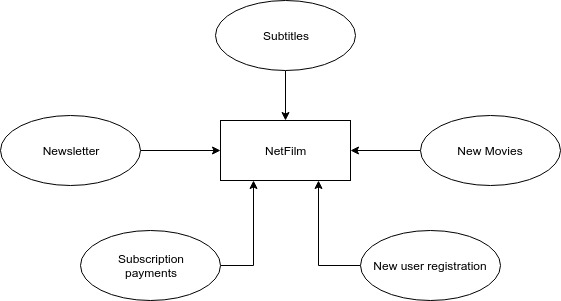
\includegraphics[width=0.8\textwidth]{img/business.jpg}
  \caption{Business Case diagram}
  \label{fig:BC}
\end{figure}

\subsection{Use cases}

In order to obtain access to the platform, one must do what follows:

\begin{itemize}
\item New user registration
\item Log in/out
\end{itemize}

User's dashboard mockup is presented in \ref{fig:UI}.
Every user shall be able to do the following things within his dashboard, after logging in:

\begin{itemize}
\item play movies
\item search movies
\item filter by genre
\item rate movie (as good or bad)
\item add movie to "My List"
\item switch to Kids mode
\item change movie settings such as resolution, language and subtitles
\end{itemize}

\begin{figure}[h]
  \centering
  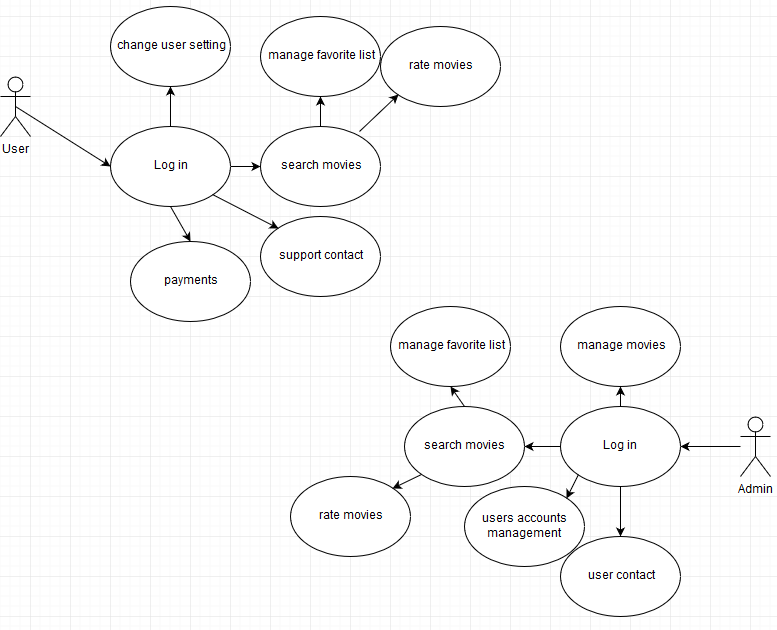
\includegraphics[width=1\textwidth]{img/usecase.PNG}
  \caption{Use Case diagram}
  \label{fig:Use case}
\end{figure}

\begin{figure}[h]
  \centering
  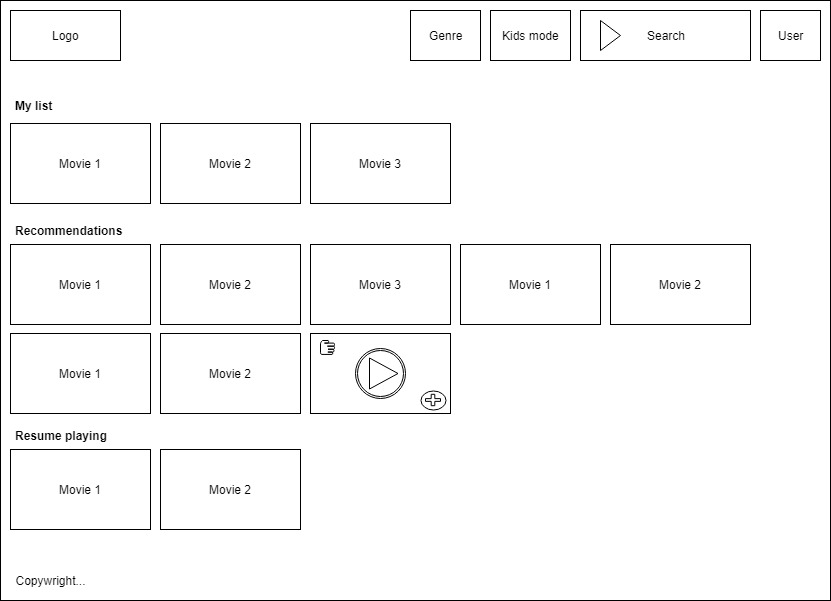
\includegraphics[width=1\textwidth]{img/UI.jpg}
  \caption{Anticipatory dashboard mockup}
  \label{fig:UI}
\end{figure}

\begin{figure}[hp]
  \centering
  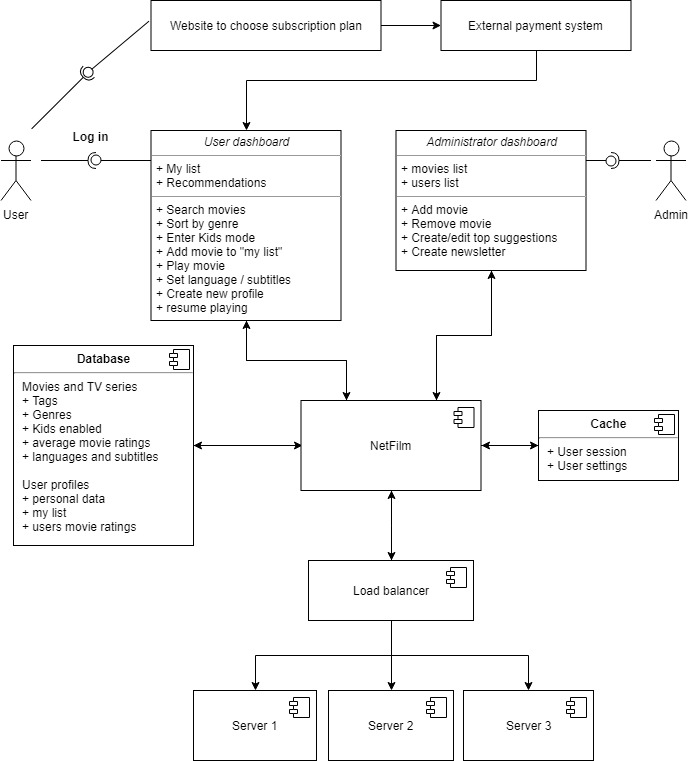
\includegraphics[width=1\textwidth]{img/sysml.jpg}
  \caption{System Requirements Diagram}
  \label{fig:SysML}
\end{figure}


\chapter{Functional Requirements}

\section{New user registration}

\subsection{Description and Priority}

In order to get system account user needs to register by giving his/her e-mail address, his/her secret password, and filling the payment information such as: 
\begin{itemize}
\item brand,
\item card number,
\item expiration date,
\item card holder,
\item CVV.
\end{itemize}

Additionally, the user have to choose subscription plan where payment for the month is in advance but the first of all subscription month is free.

Priority: \verb|high|.

\subsection{Stimulus/Response Sequences}

After clicking \verb|Register| button by user on service main screen system should redirect him/her to the registration page. There are a few fields to fill such as e-mail address, password,  payment information and selecting subscription plan. After fulfilling the form user press \verb|submit| button and is redirected to the payment service. After subscription is purchased, user receives confirmation e-mail and is encouraged to log in to his/her brand new dashboard.

\section{User login}

\subsection{Description and Priority}

In order to get into users dashboard, one needs to log in to the previously created account.

Priority: \verb|high|.

\subsection{Stimulus/Response Sequences}

After clicking \verb|Log in| button by user on service main screen system should ask him/her to provide his/her e-mail address and his/her password specified during registration process. If the verification process will be successful the user should be redirected to his/her dashboard. If verification process fails, proper information box shows up and user have another chance to correct the data. There is also option to reset the password, which results in sending new password on the given e-mail address.

\section{Play movies}

\subsection{Description and Priority}

User has to be logged in. It is necessary to play video. This feature allows to play video.

Priority: \verb|high|.

\subsection{Stimulus/Response Sequences}

According to a particular sequence to initialize video streaming user needs to press \verb|play| button that shows up when the mouse hovers on the selected movie thumbnail. As a result user will be redirected to the streaming page where video launches automatically. Additional options show up, such as audio/subtitles language selection or streaming quality selection.

\section{Search movies}

\subsection{Description and Priority}

System will allow to look for specific tags in the multimedia database.

Priority: \verb|medium|.

\subsection {Stimulus/Response Sequences}

The search engine will automatically fill in the missing letters to the matching tag and it will change to the correct page. 

\section{Filter by genre}

\subsection{Description and Priority}

Feature of system allows to seek for the movie in the database by the genre.

Priority: \verb|medium|.

\subsection{Stimulus/Response Sequences}

The \verb|genre| button reveals genre menu. User can choose any category and it will proceed to the correct page.  

\section{ Recommendation system}

\subsection{Description and Priority}


System will propose movies based on user's search history and average ratings of the movie. This will make program more pleasing for the eye.

Priority: \verb|medium|.

\subsection{Stimulus/Response Sequences}


There is no action required from user due to appearing recommendations.

\section{Rating system}
\subsection{Description and Priority}

System that allows rating of movies. There are only to options available - like or dislike.

Priority:\verb|low|.

\subsection{Stimulus/Response Sequences}

Under the movie there are two buttons- thumbs up and thumbs down. Their purpose is to rate the movie by clicking them.

\section {Add movie to "My list"}

\subsection{Description and Priority}

System that allows adding movies to user's personal list.

Priority: \verb|low|.

\subsection{Stimulus/Response Sequences}

User can add video by clicking the \verb|+| sign under the movie. This allow to add the movie to user`s personal list. 
\section{Kids mode}

\subsection{Description and Priority}

System will allow to filter movies that are kids appropriate.

Priority: \verb|low|.

\subsection{Stimulus/Response Sequences}

On the top of the page there is \verb|Kids mode| switch button that changes between Kids mode and adult mode. Clicking second time on the switch button will change the Kids mode to adult mode again.

\section{Resume playing}

\subsection{Description and Priority}

System will allow to resume partially watched video.

Priority: \verb|low|.

\subsection{Stimulus/Response Sequences}

In order to resume video user should click \verb|play| on the unfinished video. System will resume video from the last point it has been stopped. 

\chapter{Nonfunctional Requirements}

\section{Performance Requirements}

All movie streamings should be able to start within 10s over 20Mbps internet connection. When the streaming request takes longer than 5 seconds the stream will automatically end.

\section{Security Requirements}

Users shall be required to log in to the system for all operations. All network transactions that involve financial information or personally identifiable information shall be encrypted.
Additionally the search engine should be secured from the SQL injection by including function to filter characters.

\chapter{Other issues}

\section{Open Issues}
The choice of movies supplier is an important issue. The supplier can be one or several. It is depends on the service's policy.

The engine on which the service will be launched is an important issue and should be chosen in the first place. What engine will be used is not imposed drastically.

\section{Off-the-shelf solutions}

One of the ready solutions is to use popular frameworks and tools compatible with them. This will allow more efficient work and reduce the risk of project failure.

\section{New problems}

One of the problems that can occur while designing a website are the various versions of browsers available for users. There may be a problem on the client side with a frame or script that does not work due to the use of a little-popular browser.


\nocite{*}
\end{document}